\chapter{Implementation}
The delay in the network has been analysed. A protocol has been created to be utilized between the vicon and the quadcopter. Controllers for the attitude, translational velocity and position have been designed and the needed hardware, e.g. the microcontroller, have been chosen. It should thereby be possible to set up the scheduler. The scheduler should mainly handle the receiving and decoding of packets and the running of the controllers. \\ To implement the designed controllers in the scheduler, running on the micro processer, a conversion from the controllers continuous expression to a discrete expression is required.

In the following section the scheduling is described, this is followed by a section on the discretization of continuous controllers and a final section describing the implementation of the controllers on the micro processor.

\section{Scheduler}
Only two tasks are running on the microcontroller, the control algorithm and the communication. The handling of these tasks is however critical. The network introduces delays which sets a limit for the rate at which the control algorithms can be executed. It is also desirable for the control task to be executed periodically, and at any other time, the microcontroller should listen for new data on the network.\\
A scheduler can handle priorities and timing of tasks, for this purpose a real time operating system (RTOS) is used, called FreeRTOS.\\
The capabilities of this RTOS ranges beyond the needs in this project, but provides the necessary tools, and constitutes a flexible base with room for future development.\\
In \autoref{lst:scheduler} PWM and communication is initialized, the two main tasks are created with appropriate priorities, the motors are activated by a start sequence and the task scheduler is started.\\

\begin{lstlisting}[style=customcpp,
                    caption={Code for initialization, creation of the different tasks, start sequence for the motors and call to the scheduler.}, 
                    label=lst:scheduler]
int main()
{
    // Initialization
    PWM_init(0);
    USART_Init(MYUBRR);
    ADC_Init();
    
    // Task Creation
    xTaskCreate(Controllers, "Control", 1000, NULL, configMAX_PRIORITIES - 1, NULL );
    xTaskCreate(Comunication, "Com", 1000, NULL, configMAX_PRIORITIES - 2, &xHandle);
    
    // Start sequence for the motor controllers
    _delay_ms(1000);
    int duty = 128;
    Set_PWM_duty(duty, duty, duty, duty);
    _delay_ms(10000);
 
    // Scheduler Start
    vTaskStartScheduler();
    return 0;
}
\end{lstlisting}

Once the task scheduler is started the program never returns to main again. The scheduler has a configurable tick-rate, set to \SI{1}{ms}, which it uses to schedule and time tasks. The RTOS is set up to run with preemption, such that the higher priority task, controllers, can preempt the lower priority, communication, in order to achieve a periodic execution of the control algorithms. Since the XBee always sends data out on the RX-pin of the microcontroller, data will be lost if the communication is preempted. To make sure that there is always new data available for each execution of the control task, the execution frequency is chosen low enough such that at least one package is received in each period.\fxnote{make sure that this is still true after the computation time of the control algorithms has grown due to translational controllers}\\
In \autoref{fig:timingDiagram} a timing diagram is shown, but since package reception is not synchronized with the periodic control task, this is just an example.

\begin{figure}[H]
    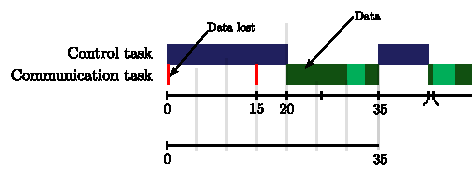
\includegraphics[width =.7\textwidth]{figures/timingDiagram}
    \centering			
    \caption{An example of task execution schedule. The control task is periodic and the packages can arrive at different instances.} 
    \label{fig:timingDiagram}
\end{figure}
\fxnote{Figure under construction - finalize figure when all execution and period times are known. Responsible: Niels}

Although the packages are received at instances unrelated to the control task, the packages still arrive periodically, though the period might fluctuate.

\section{Communication}
The communication task is used to receive the data in the microcontroller from the computer. Part of the code used can be seen in \autoref{lst:communication}.

\begin{lstlisting}[style=customcpp,
                caption={Code for the comunication task.}, 
                label=lst:communication]
void Comunication(void *pvParameters)
{
    while (1)
    {
        int pack = 0;
        pack = CheckPackageArrival();
        if (pack)
            GetPackage();
    }
    vTaskDelete(NULL);
}
\end{lstlisting}

It consist of a while loop that is running all the time and checks if a package has arrived using the function CheckPackageArrival(). This function read the bytes coming to the serial port and checks if the header is correct, returning a 0 if that is not the case. If the header was wrong, the if condition is not fulfilled and the loop starts again until it gets a correct header.

Then, the function GetPackage() reads the remaining bytes and uses the checksum to verify that the data has been sent correctly. When the summation of the parts and the checksum gives the correct value, the stored bytes are decoded and the global variables are rewritten with their new values


